%%%%%%%%%%%%%%%%%%%%%%%%%%%%%%%%%%%%%%%%%%%%%%%%%%%%%%%%%%
\usepackage[utf8]{inputenc}
\usepackage[T1]{fontenc}
%%%%%%%%%%%%%%%%%%%%%%%%%%%%%%%%%%%%%%%%%%%%%%%%%%%%%%%%%%
\usepackage{graphics}
\usepackage{graphicx}
\usepackage[graphicx]{realboxes}
\usepackage[font=small, labelfont=bf]{caption}
\usepackage{lmodern}
\usepackage{hyphenat}
\usepackage{color,colortbl}
%%%%%%%%%%%%%FIXED ORDER%%%%%%%%%FIXED ORDER%%%%%%%%%%%%%%
%\usepackage[top=2.5cm,left=3cm,right=2.5cm,bottom=2.5cm]{geometry}
%%%%%%%%%%%%%%%%%%%%%
\usepackage[portuguese]{babel}
\usepackage{scrbase}
\usepackage{babelbib}
%%APPENDIX SETTINGS%%
\usepackage[title, toc, titletoc, page]{appendix}
\usepackage[toc, page]{appendix}
%%%%%%%%%%%%%%%%%%%%%
\usepackage{subcaption}
\usepackage{verbatim}
\usepackage{pgfgantt}
\usepackage{url}
\usepackage{listings}
\usepackage[calc, en-US]{datetime2}
\usepackage{etoolbox}
\usepackage{xparse}
%%%%%%%%%%%%%%%%%%%%%%%%%%%%%%%%%%%%%%%%%%%%%%%%%%%%%%%%%%
%\usepackage[nottoc]{tocbibind}
%\usepackage[shortcuts, nopostdot, acronym, toc, nogroupskip, nonumberlist, automake]{glossaries}
%\usepackage[usenames, dvipsnames, svgnames, table]{xcolor}
%\usepackage[hidelinks]{hyperref}
%%%%%%%%%%%%%%%%%%%%%%%%%%%%%%%%%%%%%%%%%%%%%%%%%%%%%%%%%%
\usepackage{multicol}
\usepackage{makecell}
\usepackage{array}
\usepackage{tabularx}
\usepackage[export]{adjustbox}
\usepackage{eurosym}
\usepackage{float}
%%%%%%%%%%%%%%%%%%%%%%%%%%%%%%%%%%%%%%%%%%%%%%%%%%%%%%%%%%
\usepackage{amsmath}
\usepackage{amsfonts}
\usepackage{amssymb}
\usepackage{mathrsfs}
\usepackage{paralist}
\usepackage{enumerate} %%conflict never put enumitem with enumerate
%\usepackage{enumitem} %%conflict never put enumitem with enumerate
\usepackage{multirow}
\usepackage{lscape}
%%%%%%%%%%%%%%%%%%%%%%%%%%%%%%%%%%%%%%%%%%%%%%%%%%%%%%%%%%
\usepackage{scrhack}
\usepackage{longtable}
\usepackage{booktabs}
\usepackage[autostyle=true]{csquotes}
\usepackage{calc}
\usepackage{siunitx}
\usepackage{setspace}
%\usepackage{titlepic}
%%%%%%%%%%%%%%%%%%%%%%%%%%%%%%%%%%%%%%%%%%%%%%%%%%%%%%%%%%
\usepackage{lipsum}
%%%%%%%%%%%%%%%%%%%%%%%%%%%%%%%%%%%%%%%%%%%%%%%%%%%%%%%%%%
\usepackage{moreverb}
\usepackage{rotating}
%%%%%%%%%%%%%%%%%%%%%%%%%%%%%%%%%%%%%%%%%%%%%%%%%%%%%%%%%%
\usepackage{romannum}
%\usepackage{tikz}
%\usepackage{circuitikz}
%\usetikzlibrary{matrix, shapes.geometric, arrows, trees, positioning, calc}
%%%%%%%%%%%%%%%%%%%%%%%%%%%%%%%%%%%%%%%%%%%%%%%%%%%%%%%%%%%%%%%%
\usetheme{Frankfurt}
%\makeindex
%%%%%%%%%%%%%%%%%%%%%%%%%%%%%%%%%%%%%%%%%%%%%%%%%%%%%%%%%%%%%%%%
%\bibliographystyle{plain}
%\bibliographystyle{ieeetr}
%\selectbiblanguage{portuguese}
%\setbtxfallbacklanguage{english}
%%%%%%%%%%%%%%%%%%%%%%%%%%%%%%%%%%%%%%%%%%%%%%%%%%%%%%%%%%%%%%%%
\begin{document}
\begin{frame}
\frametitle{Plano de Desenvolvimento}
\begin{minipage}{.5\linewidth}
\begin{figure}[ht]
\begin{flushleft}
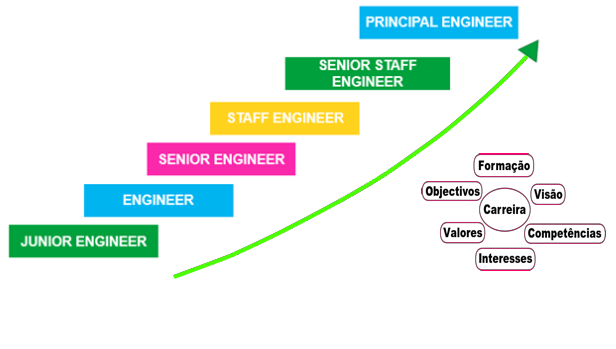
\includegraphics[scale=0.35]{./image/Career_Path/Progressao.png}
\end{flushleft}
\end{figure}
\end{minipage}
\begin{minipage}{.45\linewidth}
\begin{figure}[ht]
	\begin{flushleft}
		
\includegraphics[scale=0.25]{./image/Career_Path/Old_Age.jpeg}
	\end{flushleft}\vfill
	\begin{flushright}
		
\includegraphics[scale=0.1]{./image/Career_Path/Burial.jpeg}
	\end{flushright}
\end{figure}
\end{minipage}
\vfill
\hfill {\tiny Sérgio Santos}
\end{frame}
%\maketitle
%%%%%%%%%%%%%%%%%%%%%%%%%%%%%%%%%%%%%%%%%%%%%%%%%%%%%%%%%%%%%%%%%%%%%%%%%%%%%%%%%%%%%%%%%%%%%%%%%%%%%%%%%%%%%%%
%\begin{frame}{Nome da Organização}
%\tableofcontents
%\end{frame}
%%%%%%%%%%%%%%%%%%%%%%%%%%%%%%%%%%%%%%%%%%%%%%%%%%%%%%%%%%%%%%%%%%%%%%%%%%%%%%%%%%%%%%%%%%%%%%%%%%%%%%%%%%%%%%%
\AtBeginSection[]{
\begin{frame}
\frametitle{Conteúdo}
\tableofcontents[currentsection]
\end{frame}}
%%%%%%%%%%%%%%%%%%%%%%%%%%%%%%%%%%%%%%%%%%%%%%%%%%%%%%%%%%%%%%%%%%%%%%%%%%%%%%%%%%%%%%%%%%%%%%%%%%%%%%%%%%%%%%%
\section{Mercado de Trabalho}
%%%%%%%%%%%%%%%%%%%%%%%%%%%%%%%%%%%%%%%%%%%%%%%%%%%%%%%%%%%%%%%%%%%%%%%%%%%%%%%%%%%%%%%%%%%%%%%%%%%%%%%%%%%%%%%
\begin{frame}
\frametitle{\textcolor{green}{O que é dinheiro ?}}
\textsc{\large Dinheiro é uma representação de valore, é o teu trabalho, os teus valores e competências, tudo que representas a não ser que sejas político.}\\
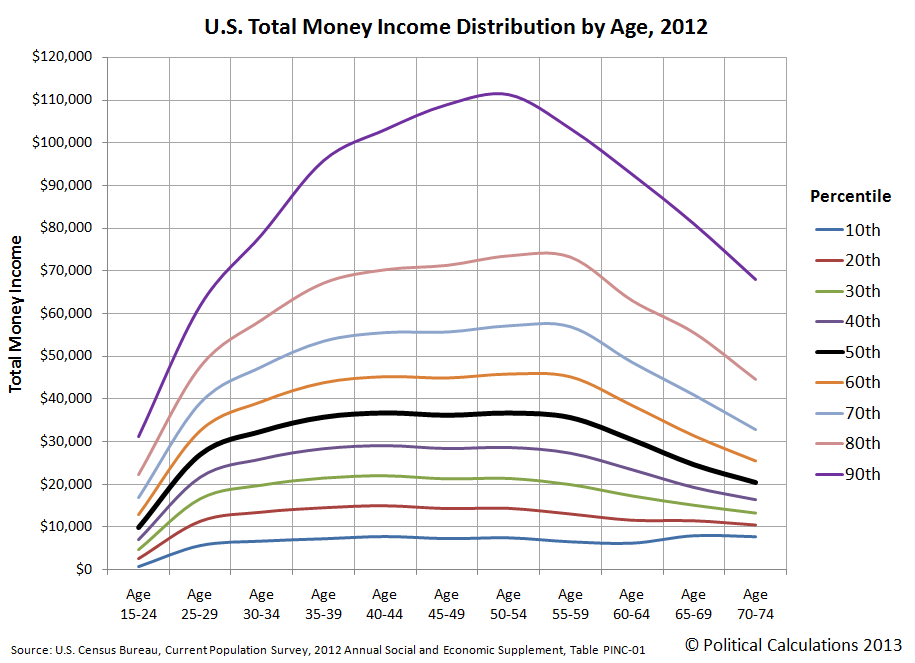
\includegraphics[scale=0.2]{./image/Career_Path/Income_2012}\hspace{0.8cm}
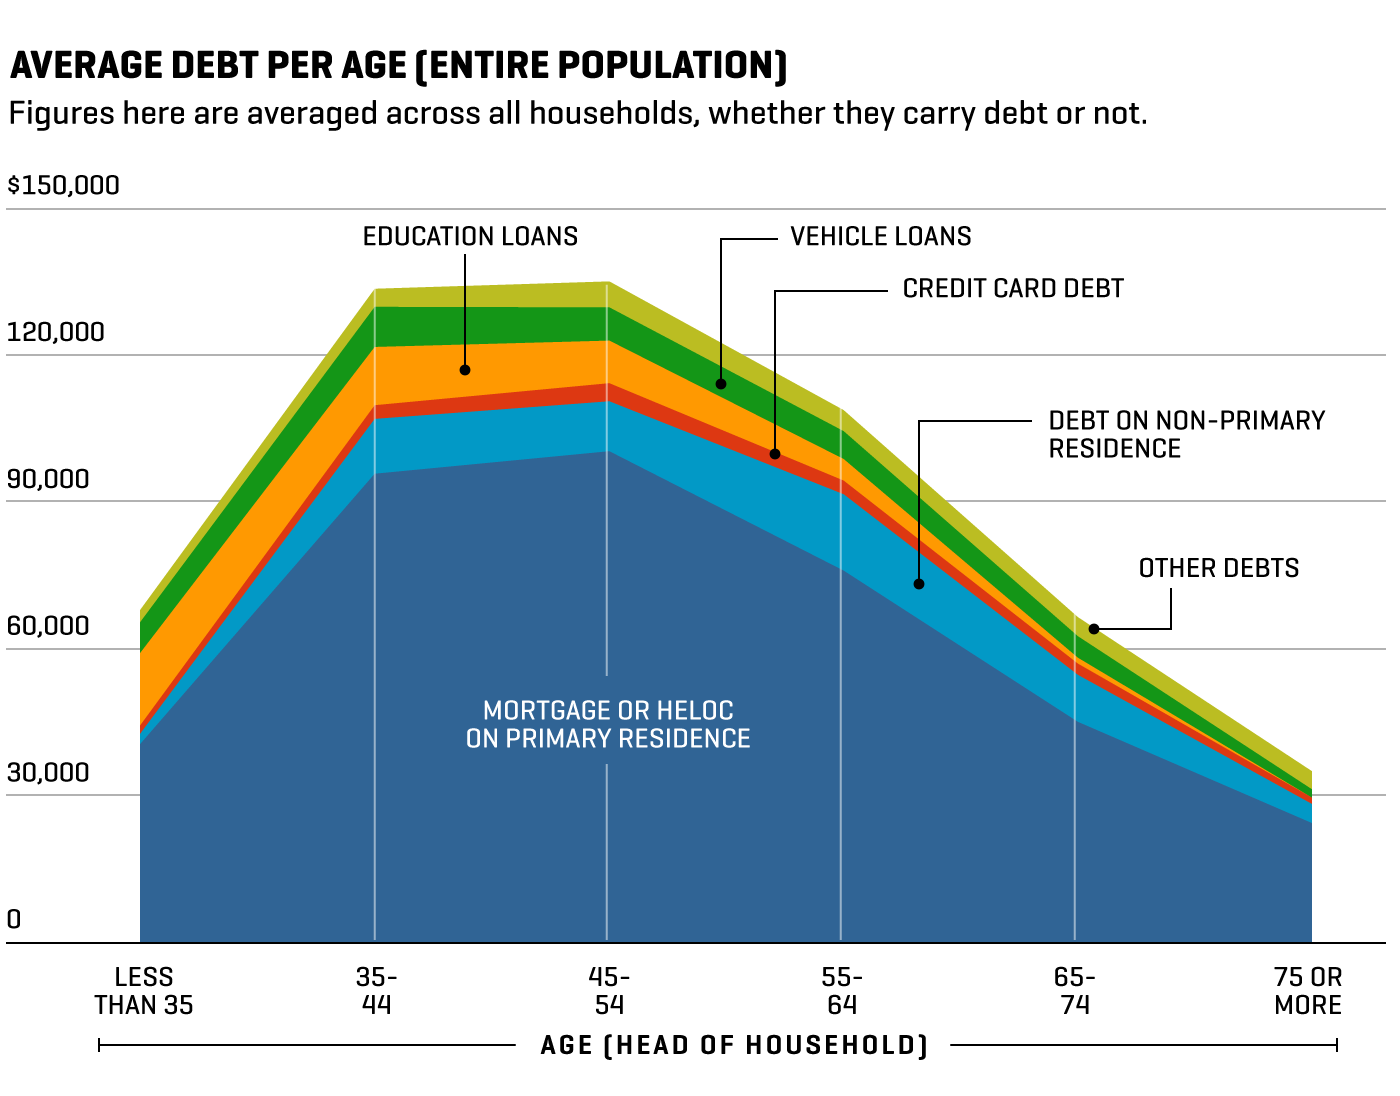
\includegraphics[scale=0.125]{./image/Career_Path/Debt}
\end{frame}
%%%%%%%%%%%%%%%%%%%%%%%%%%%%%%%%%%%%%%%%%%%%%%%%%%%%%%%%%%%%%%%%%%%%
\begin{frame}
\frametitle{\textcolor{green}{Porque Dinheiro ?}}
\begin{itemize}
	\item \textbf{Portabilidade} \\
	Reconhecido internacionalmente, sendo que cada pais tem uma cotação de valore de mercado, sendo o Pound, Dólar ,Euro e Yuan as mais fortes, em ordem decrescente, e o dólar a moeda de cambio internacional até agora.
	\item \textbf{Avaliação} \\
	Por isso que na escola os teus resultados são notas.\\
	Portugal pertence a Europa, mas um Português tem menos valor que um Alemão, Francês, Italiano e Espanhol, a não ser que sejas Político Português.\\Um Euro vale 7,69 Yuan, pelo menos um chinês vale sete vezes menos que um Europeu.\\
	\item \textbf{Modernização} \\
	Das cavernas a sobreviver do ambiente, a troca de bens, e ao cambio por moeda.
\end{itemize}
\end{frame}
%%%%%%%%%%%%%%%%%%%%%%%%%%%%%%%%%%%%%%%%%%%%%%%%%%%%%%%%%%%%%%%%%%%%
\begin{frame}
\frametitle{Valorização Pessoal}
\begin{center}
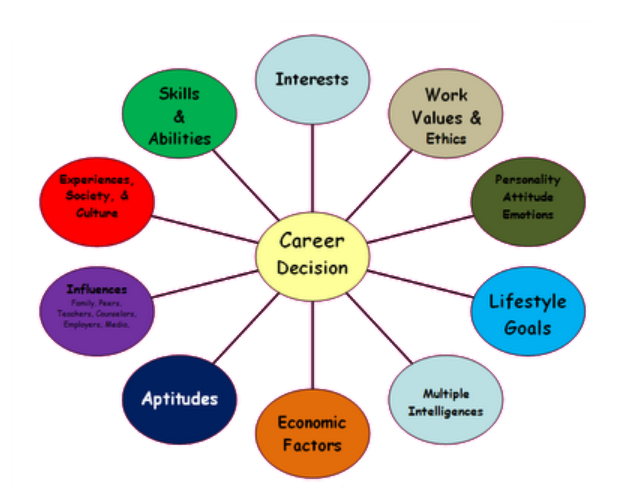
\includegraphics[scale=0.4]{./image/Career_Path/Career_Decision_Factors}
\end{center}
\end{frame}
\section{Plano de Desenvolvimento}
%%%%%%%%%%%%%%%%%%%%%%%%%%%%%%%%%%%%%%%%%%%%%%%%%%%%%%%%%%%%%%%%%%%%
\begin{frame}
\begin{minipage}{16cm}
	\textbf{Metodologias da gestão}:\\
	\\
	\begin{minipage}{8cm}
		Instrumental
		\begin{enumerate}
			\setlength\itemsep{1.5em}
			\item Planear
			\item Organizar
			\item Controlar \\
		\end{enumerate}
	\end{minipage}
	\begin{minipage}{5cm}
		Comportamental
		\begin{enumerate}
			\setlength\itemsep{.5em}
			\item Liderança
			\item Comunicação
			\item Motivação
			\item Tomada de decisão
		\end{enumerate}
	\end{minipage}
\end{minipage}
\end{frame}
%%%%%%%%%%%%%%%%%%%%%%%%%%%%%%%%%%%%%%%%%%%%%%%%%%%%%%%%%%%%%%%%%%%%
\begin{frame}
\textbf{\Large Competências:}\\
\begin{minipage}{15cm}
	\begin{figure}[ht]
		\centering
		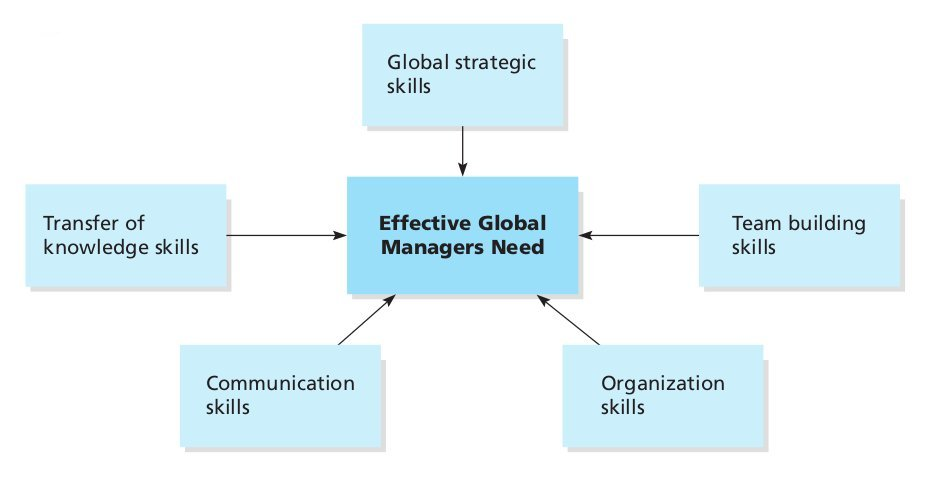
\includegraphics[scale=0.3]{./image/Skills/Managerial_Skills_for_the_Global_Marketplace.jpg}
	\end{figure}
\end{minipage}
\end{frame}
%%%%%%%%%%%%%%%%%%%%%%%%%%%%%%%%%%%%%%%%%%%%%%%%%%%%%%%%%%%%%%%%%%%%
\begin{frame}
Depois disso tudo, temos de fazer marketing pessoal e adquirir um trabalho. \vfill
\begin{minipage}{5cm}
	\begin{figure}[ht]
		\flushleft
		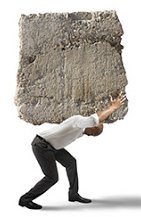
\includegraphics[scale=0.6]{./image/Job/Burden.jpg}
	\end{figure}
\end{minipage}
\end{frame}
%%%%%%%%%%%%%%%%%%%%%%%%%%%%%%%%%%%%%%%%%%%%%%%%%%%%%%%%%%%%%%%%%%%%
\section{Conclusões}
\begin{frame}
\begin{minipage}{7cm}
	\begin{figure}[ht]
		\flushleft
		
\includegraphics[scale=0.7]{./image/Objectives/Meaning_of_Life.jpeg}
	\end{figure}
\end{minipage}
\begin{minipage}{5cm}
	\begin{itemize}
		\item Eat, Sleep, Do what you enjoy.
		\item Do not be exploited.
		\item See things has they are.
		\item Grow and become a better person.
		\item Relax, Value yourself.
		\item Confidence.
		\item Make it up has you go along.
	\end{itemize}
\end{minipage}
\end{frame}
%%%%%%%%%%%%%%%%%%%%%%%%%%%%%%%%%%%%%%%%%%%%%%%%%%%%%%%%%%%%%%%%%%%%
\end{document}
%%%%%%%%%%%%%%%%%%%%%%%%%%%%%%%%%%%%%%%%%%%%%%%%%%%%%%%%%%%%%%%%%%%%